\section{Application Scenarios}
\label{sec:caseStudy}
% \shusen{A full case study that driven by the visualization task and the question associated with them}
%In this section, we discuss application scenarios, in which the domain experts utilize the
To better illustrate how the proposed perturbation-driven exploration tool helps researchers interpret the neural network model, we present five application scenarios gathered by the domain experts who integrated the proposed tool into their analysis workflow.


\subsection{Scenario 1: Assess the Model Prediction Stability}
The robustness of the prediction is often hard to evaluate, however, they provide valuable information for the researchers to better understand the model.
%
In the proposed work, we approach the prediction robustness from sensitivity analysis point of view. The stability of the prediction is measured by how often the predicted labels are altered after small perturbations are applied to the input.
%
Compare to other types of input (e.g., image), perturbation of the natural language can be particular tricky, as small alteration of words can drastically change the meaning of the sentence. As discussed in Section~\ref{sec:sentence}, we try to maintain semantic of the sentence by only replace words with their synonymous and only replace one word for each pair.
As illustrated in Fig.~\ref{fig:predictStability}, by utilizing the proposed tool, the domain expert can not only examine visual summary of the stability, but also quickly dive into individual examples for case by case analysis.

\begin{figure}[htbp]
\centering
\vspace{-2mm}
 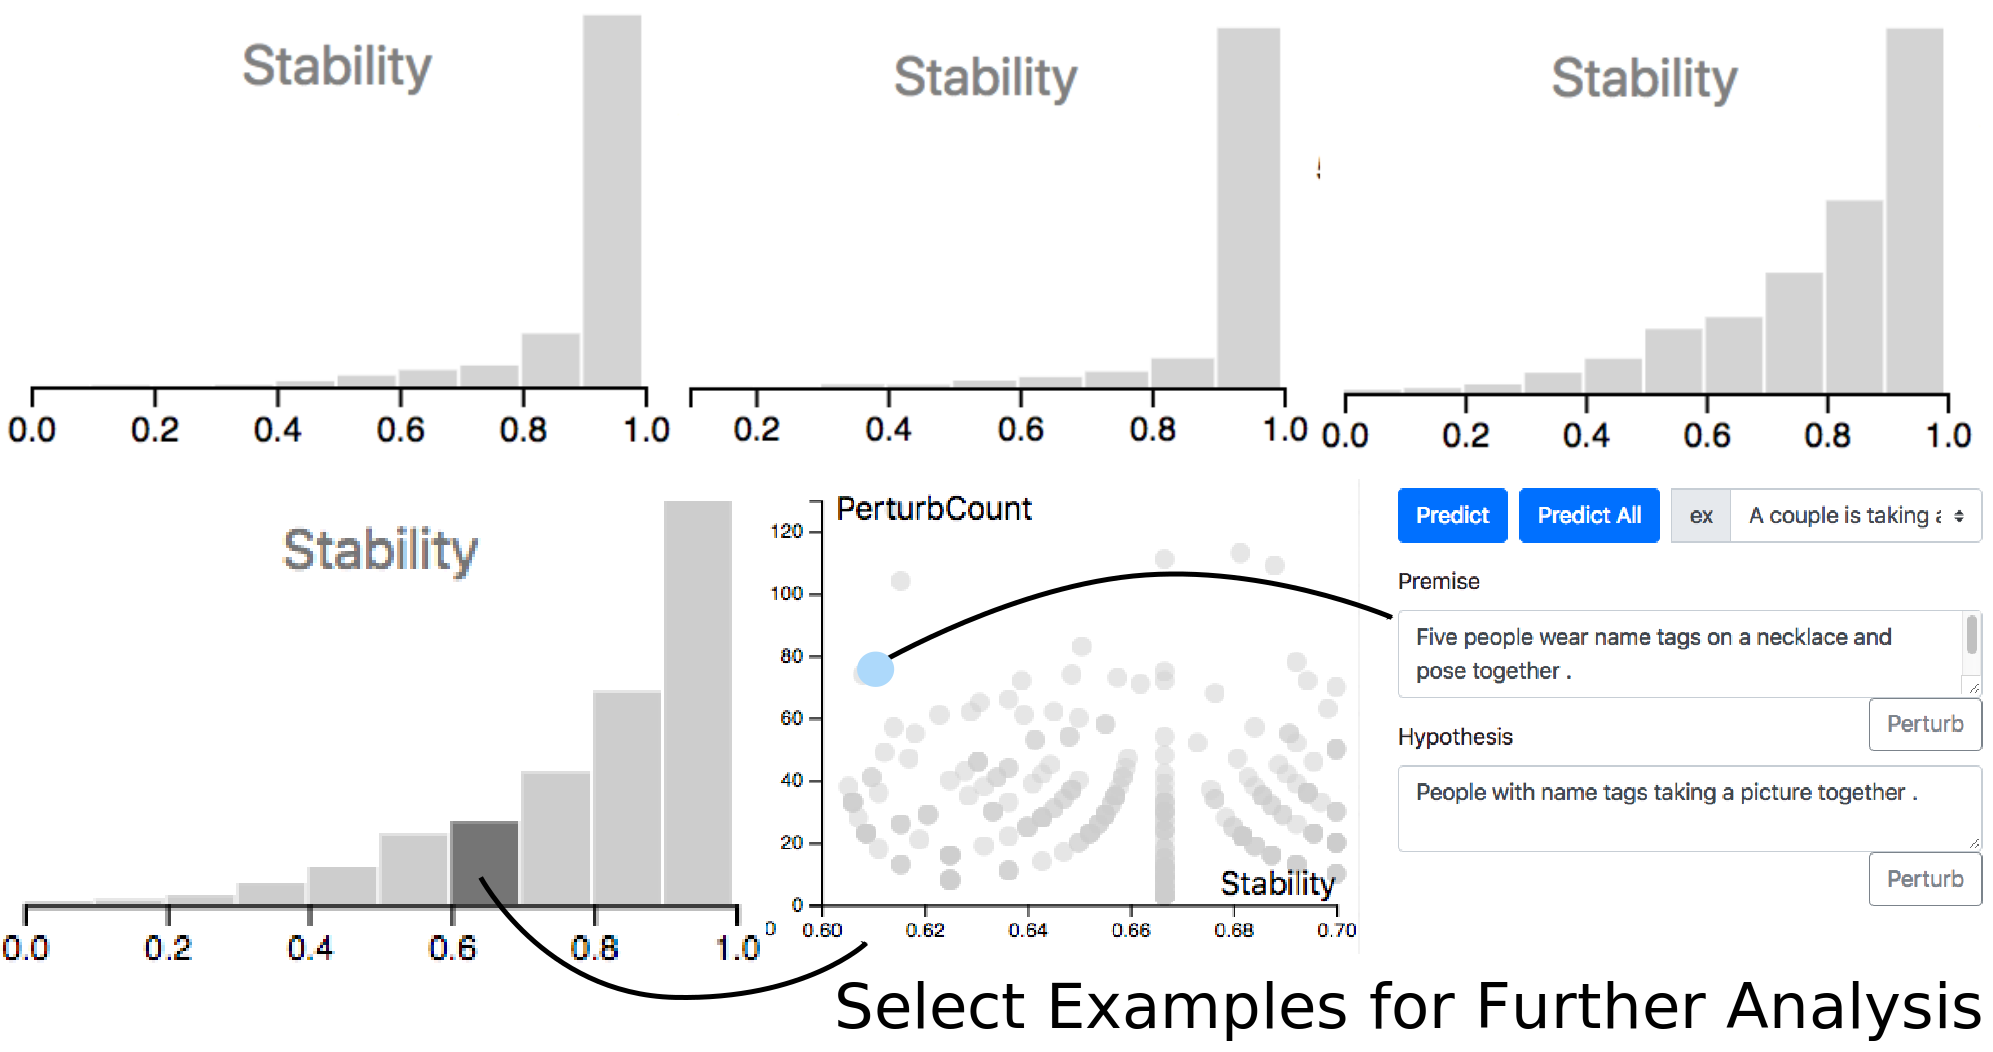
\includegraphics[width=1.0\linewidth]{predictStability}
 \vspace{-4mm}
 \caption{
Prediction stability assessment. In (a)(b)(c), we estimate the overall prediction stability (regarding synonymous perturbation) for each type prediction over the entire development set (10k examples). The user can drill down to individual examples by filtering via the histogram or scatterplot (see Fig.~\ref{fig:summaryView}). For highly unstable prediction, we often observe the original prediction is near a decision boundary (e.g., the yellow circle in (e) corresponds to a prediction that is at the boundary between \emph{entailment} and \emph{neutral}), however, some predictions, such as the one illustrated in (d) can alter the prediction quite drastically with minor perturbation (illustrated in $d_1$, where the word ``pile'' is replace by ``heap'' in the hypothesis sentence).
}
\label{fig:predictStability}
\vspace{-2mm}
\end{figure}

In Fig.~\ref{fig:predictStability}(a)(b)(c),  %by viewing the distribution of the stability in the histogram
we compare the overall prediction stability (regarding synonymous perturbation) for each type prediction over the entire development set (10k examples).
%
We observe a drastic difference between the stability for entailment predictions compare to the contradiction and neutral ones.
%
Such a distinction can be partially explained by how entailment relationship is defined. As discussed in the Section~\ref{sec:languageInference}, the relationship is only valid if the concept in premise is more specific than the concept in hypothesis (therefore, you can infer the hypothesis from the premise, but not other way around). This means, we may change the entailment relationships simply by replacing nouns and verb by synonymous, whereas, the same does not apply for neutral and contradiction.
%
The inherent sensitivity difference may motivate domain experts designing dedicate model mechanism to address the such a disparity.

Beside presenting the summary view, the tool also allow user to quickly narrow down the select to single example  by filtering through the histogram and scatterplot (see Fig.~\ref{fig:summaryView}).
%
Through exploring multiple samples (in the entailment category, E/E in Fig.~\ref{fig:summaryView}(a)), the domain experts noticed many highly unstable outliers are from sentence pairs where the prediction is near the decision boundary (see Fig.~\ref{fig:predictStability}(e), the yellow circle corresponds to a \emph{entailment} prediction that is very close to \emph{neutral}).
However, some predictions, such as the one illustrated in Fig.~ref{fig:predictStability}(d) can alter the prediction quite drastically with minor perturbation (illustrated in $d_1$, where the word ``heap'' is replace by ``pile'' in the hypothesis sentence. We will try to understand the what is happened inside the model in the following section (see Fig.~\ref{fig:att2pred}).

%%%%%%%%%%%%%%%%%%%%%%%%%%%%%%%%%%%%%%%%%%%%%%%
% perturb input, attention
\subsection{Scenario 2: Examine the Decision Making Process}
The predicted label alone provide limited information. Often, domain experts want to know how does the model arrive at such a conclusion. And if the prediction is incorrect, where does the error occur in the model?
%
Examining the decision making process is not only instrumental for evaluating the model performance but also essential for hypothesizing improvement strategies for developing future models.
%
In the NLI model, the three stages (encoder, attention, classifier) work in synergy to produce the prediction.
Therefore, making sense of the prediction involves understanding how different parts of the model affect the final prediction.

In the previous section, we have noticed some unexpected behavior, where a minor perturbation of the text from \emph{pile} to \emph{heap} lead to change in the final prediction label (Fig.~\ref{fig:predictStability}(d)). Here, we want to make sense of what lead to the failed prediction. In this particular example, the premise \textbf{P} is ``A very young child in a red plaid coat and pink winter hat makes a snowball in a large \textbf{pile} of snow.'', and the original hypothesis \textbf{H1} is ``A child in a red plaid coat and pink winter hat makes a snowball in a large \textbf{pile} of snow.''. The perturbed hypothesis \textbf{H2} replaces the word \textbf{pile} with \textbf{heap}.

As illustrated in Fig.~\ref{fig:att2pred}(a), based on the graph attention visualization, we can see in the attention for (\textbf{P}, \textbf{H2}) pair, the word \textbf{pile} and \textbf{heap} is not well-aligned (see Fig.~\ref{fig:att2pred}(a)).
%
To verify whether the alignment is what contribute to the misclassification, the domain expert utilize the attention editing functionality in the matrix view (Fig.~\ref{fig:attView}) to make the word \textbf{pile} align with \textbf{heap} (shown in Fig.~\ref{fig:att2pred}(b)).
%
In the update prediction view (see Fig.~\ref{fig:att2pred} (d)), we can see the editing of attention lead to changes in prediction. The original prediction moved from neutral toward the entailment (which is the true label) and straddle on the class boundary. However, the correct alignment does not full fix the prediction problem as the original pair (\textbf{P}, \textbf{H1}) is clearly predicted as \emph{entailment} (as showed in Fig~\ref{fig:predictStability}(d)).
%
Interestingly, the original pair's attention is almost identical to the edited attention (the comparison is not shown in the figure). Such an observation means that the model do not strongly believe ``\textbf{heap} of snow'' and ``\textbf{pile} snow'' has the same meaning, which indicate the potential issue with encoder or word embedding.

\begin{figure}[htbp]
\centering
\vspace{-2mm}
 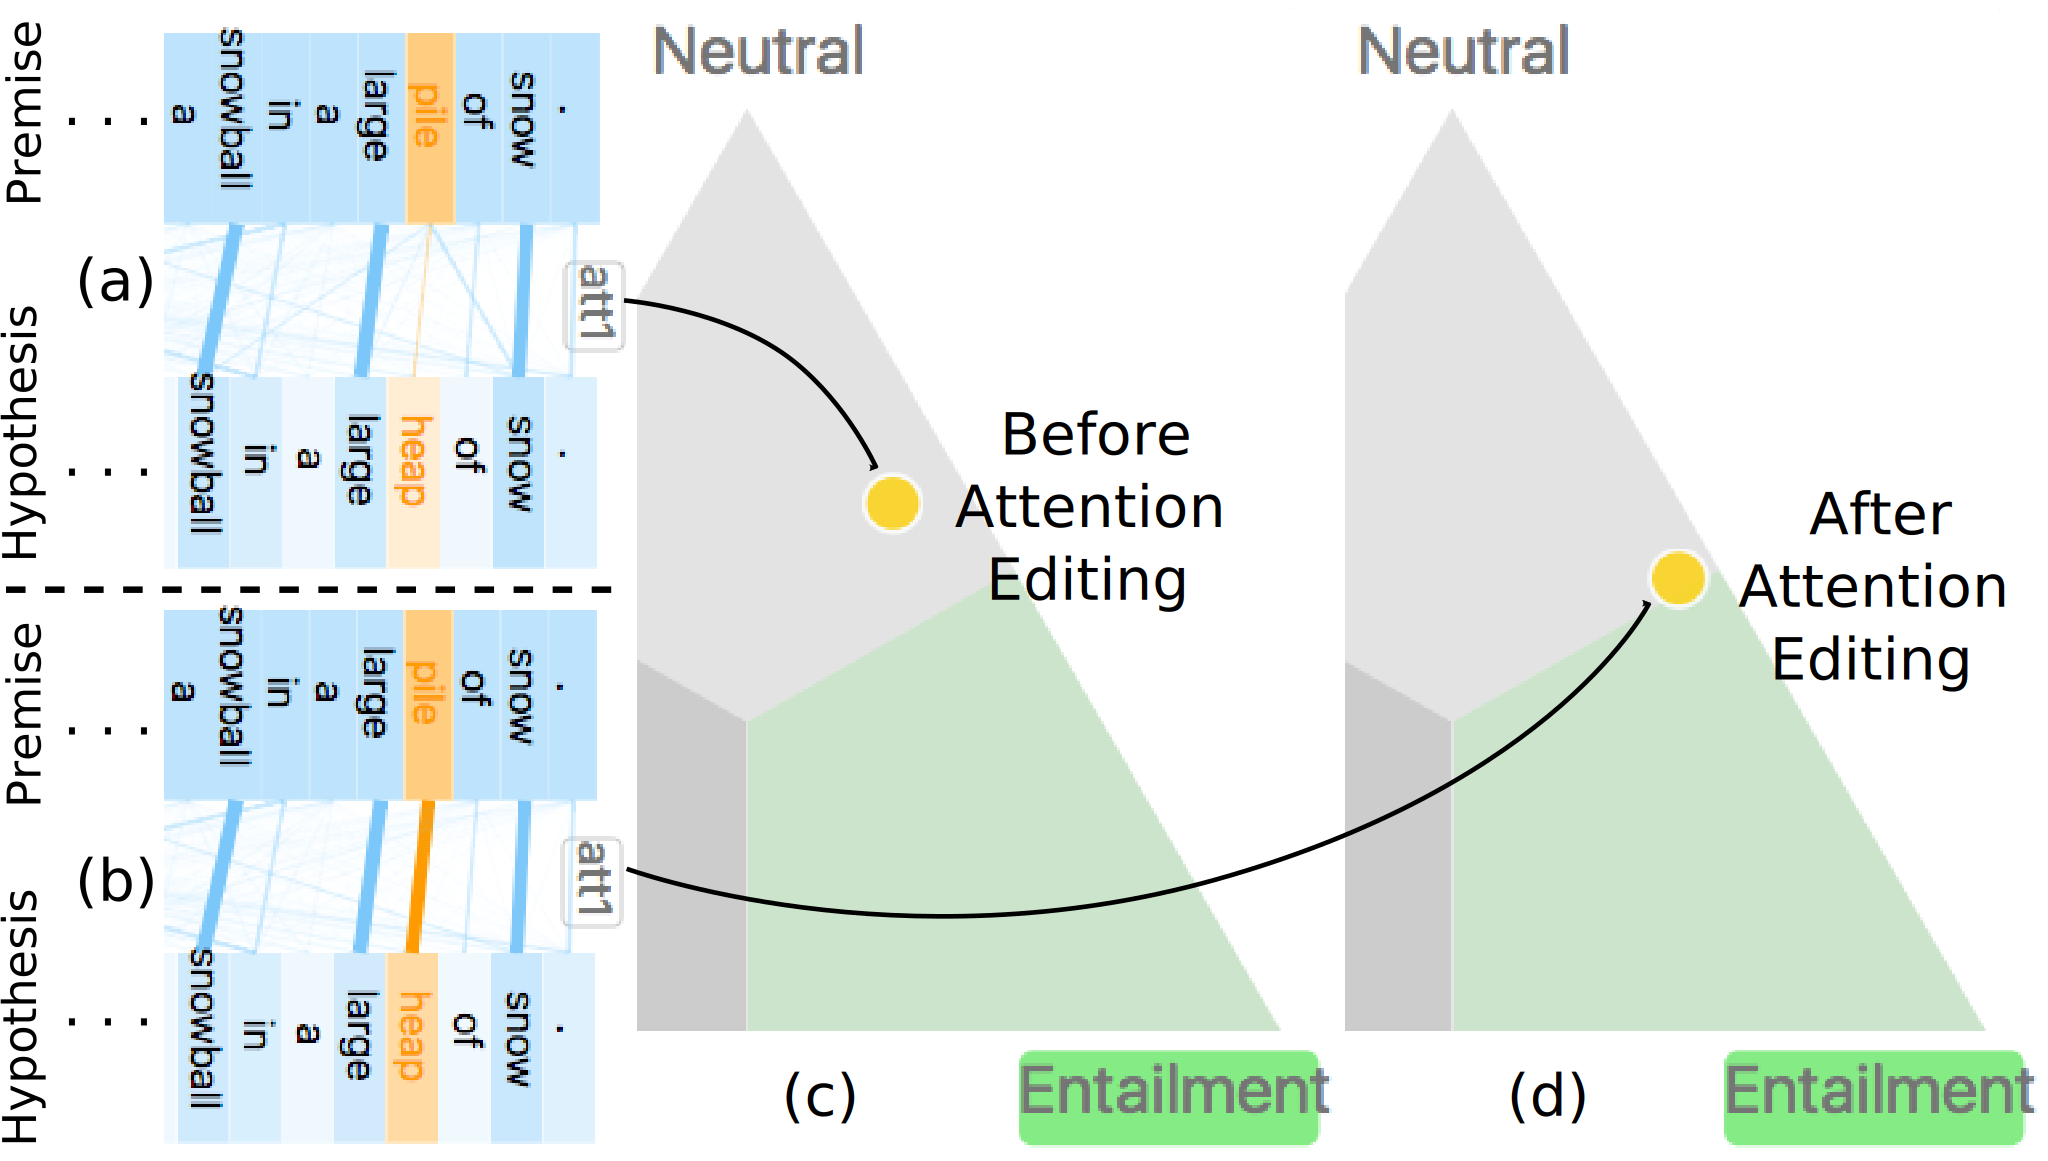
\includegraphics[width=1.0\linewidth]{att2pred}
 \caption{
Editing the original attention (a) to correctly align the word "heap" with "pile" as shown in (b) (these two words are highlight in orange).
The change of attention lead to change of prediction from neutral to the class boundary between neutral and entialment.
%
}
\label{fig:att2pred}
\end{figure}

%\shusen{Example where the prediction is correct but the alignment is wrong}
%%%% are we obtain correct prediction from wrong alignment %%%%%
%By looking into the model decision making process, we can assess whether the model is behaving as intended. For the attention based NLI model, one underlying assumption is that the attention should capture the correct alignment between words in the premise and hypothesis sentence for the classifier to make an informed/correct decision.
In the previous example, we show that even the alignment is perfect, the model still does not generate a correct prediction.
However, as illustrated in Fig.~\ref{fig:wrongAlignRightPred}, it is also likely that model produce correct predictions from the wrong attention (i.e., the important words are mis-align). The word \textbf{break} and \textbf{sit} should not align with each other (Fig.~\ref{fig:wrongAlignRightPred}(a)), however, it still produce the correct \emph{neutral} label (Fig.~\ref{fig:wrongAlignRightPred}(b)).

\begin{figure}[htbp]
\centering
\vspace{-2mm}
 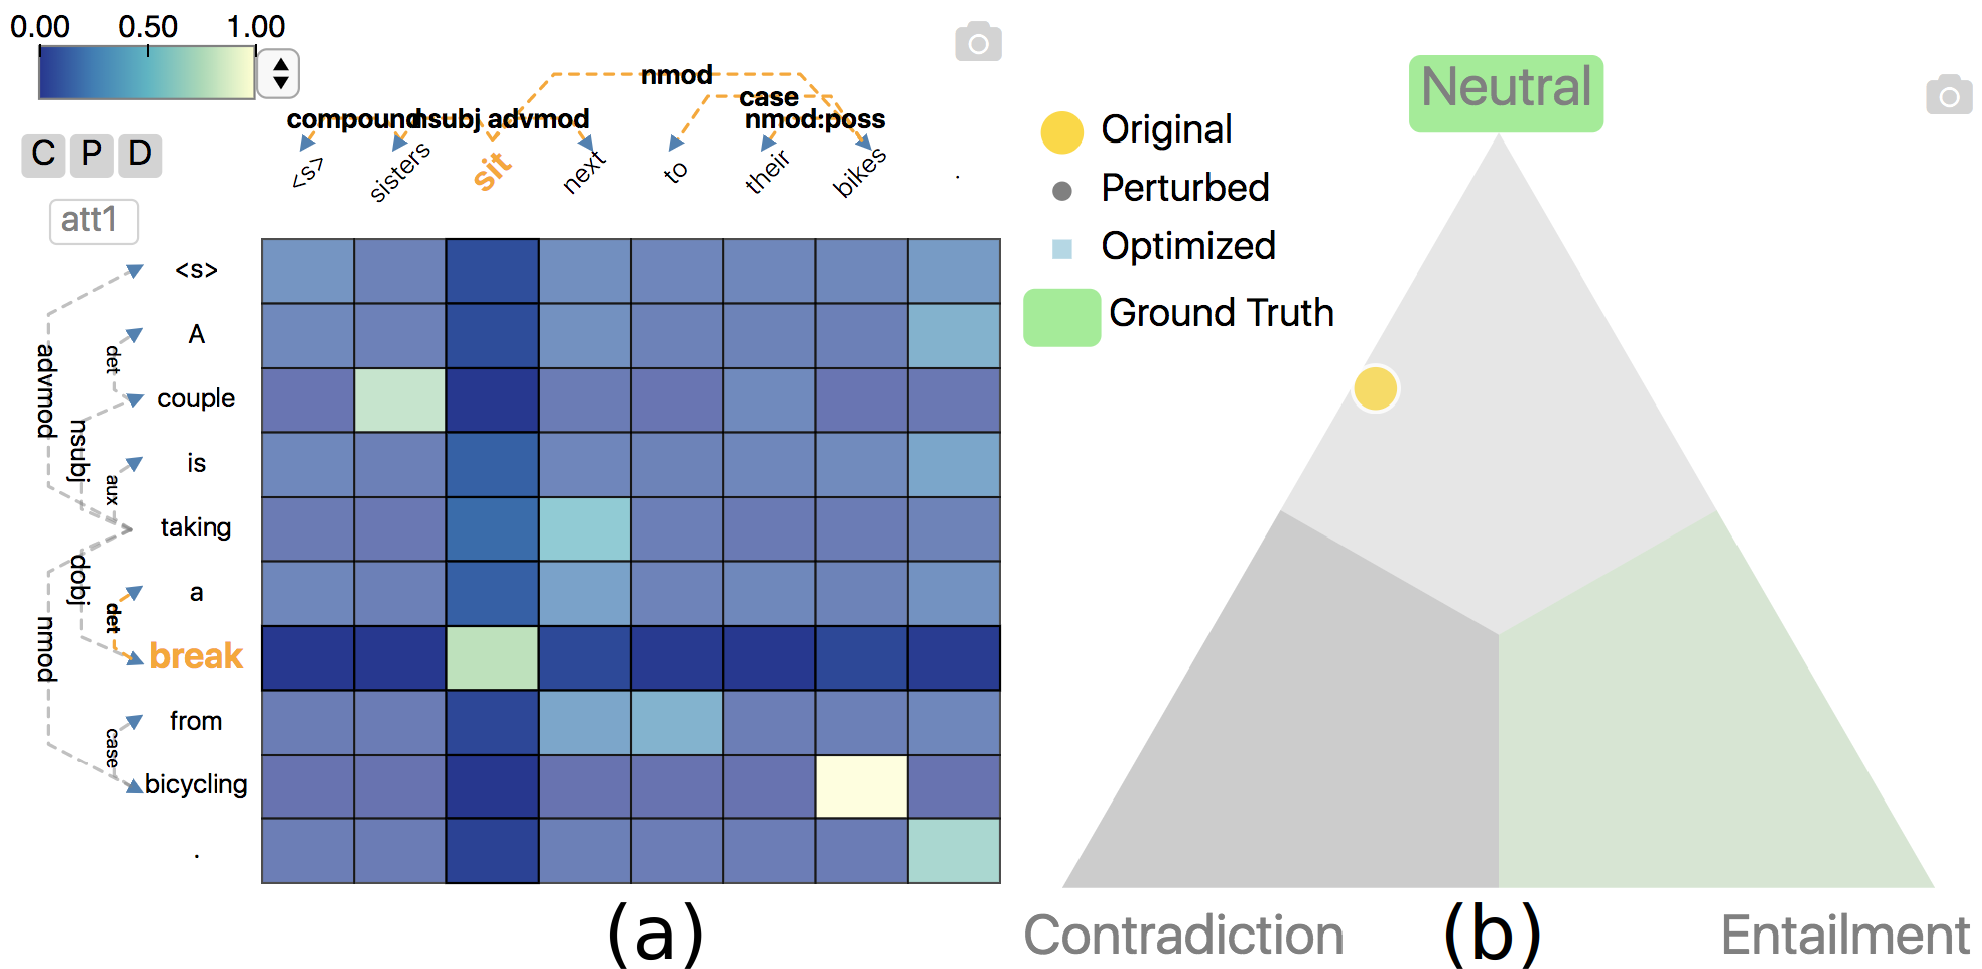
\includegraphics[width=1.0\linewidth]{wrongAlignRightPred}
 \caption{
The example of model producing right prediction with wrong attention.
The word \textbf{break} and \textbf{sit} should not align with each other (a), yet, it still yield the correct prediction (b).
}
\label{fig:wrongAlignRightPred}
\end{figure}


%%%% hypothesis on which part of model is wrong? %%%%%


%One of the essential task for can be made in either of these stages.
% \shusen{difference in sensitivity among entail natural and contradict relationships}
% the generate the correct prediction for the wrong reason


%%%%%%%%%%%%%%%%%%%%%%%%%%%%%%%%%%%%%%%%%%%%%%%
\subsection{Scenario 3: What Does It Take to Correct a Failed Prediction?}
Up till now, we have employed perturbation for input to understand prediction robustness, utilized the perturbation of attention to infer the model decision making process. Both these perturbation operations rely on forward propagation in the pipeline and assume the model parameter stay unchanged.
%
However, once we get a sense of how predictions are being made and hypothesized about the cause of failure in case of a prediction error, it nature to ask the follow up question, what does it take to fix an incorrect prediction? And more importantly, what role does each of the three stages play in such a process, are they affect the prediction differently?

Domain experts obtain answers to these questions by utilizing the prediction and pipeline view in the proposed. As discussed in details in Section~\ref{sec:pipelineView}, we employed an margin-infused relaxed algorithm (MIRA) based optimization with two complementary objectives (1. apply least amount of change to the parameter, 2. making the new prediction as close to the reassigned prediction as possible) to update the network parameters.
%
We can then visualize how much each stage of the model is changed through the distribution of parameters change.

To infer the role each stage of the pipeline plays, the proposed tool allow the parameter update to be enabled or disabled for each pipeline stage.
The tool also includes an automatic option to try all the possible combination configurations. As illustrated in Fig.~\ref{fig:pipelineUpdate}, the ground truth for this sentence pair is neutral. However, the model produces an incorrect label entailment. We reassign the prediction to neural, which triggers model update optimization for $7$ different pipeline configurations. Four configurations are shown in Fig.~\ref{fig:pipelineUpdate}(a)(b)(c)(d), the arrow line highlights the corresponding prediction for each of the update model.

Interestingly, all configurations except one are concentrated around the full neural prediction. Referring back to the pipeline visualization, we can see the one configuration that failed to produce the correct label is when only attention stage update is allowed.
%
In other words, update of attention stage seems to have significant less impact on the prediction result compared to the classifier or encoder of the model.
%The attention layer is less sensitive compared to encoding layer and classification layer.
We also examined many other sentences pairs, such an observation remains.
%This gives domain expert some hint about the significance of the role of each pipeline stage play in this model.
% which based on the natural extension of the margin-infused relaxed algorithm (MIRA) to the neural network generalize the concept of maligin combined effort of the  proposed technique

%
%However, to understand how the model should



\begin{figure*}[t]
\centering
\vspace{-2mm}
 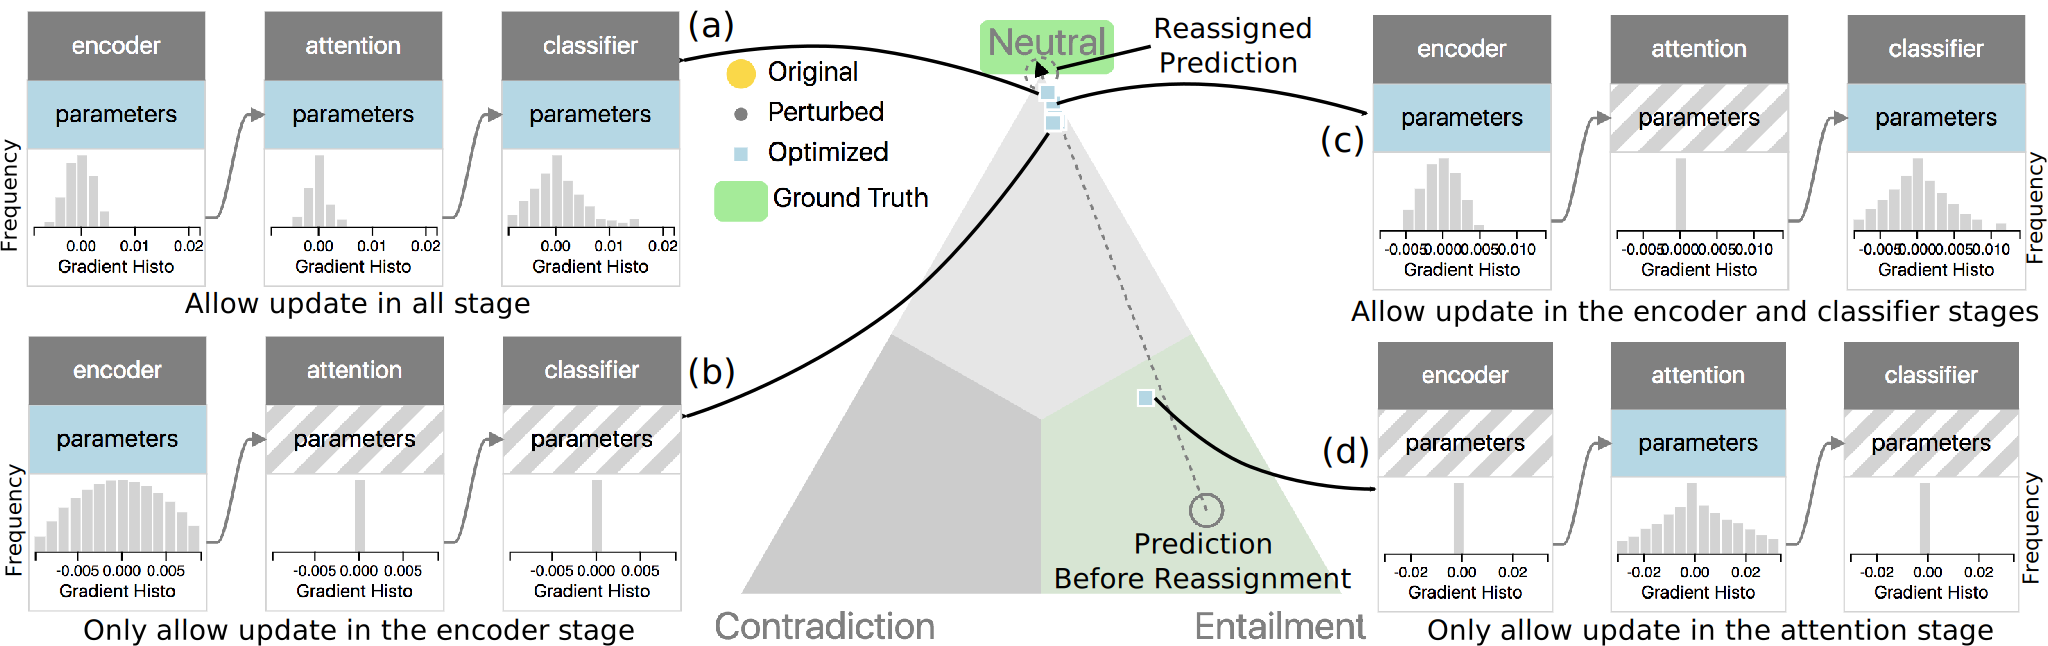
\includegraphics[width=1.0\linewidth]{pipelineUpdate}
 \caption{
How changes in different stage impact the prediction.
 }
\label{fig:pipelineUpdate}
\end{figure*}

%%%%%%%%%%%%%%%%%%%%%%%%%%%%%%%%%%%%%%%%%%%%%%%
\subsection{Scenario 4: Explore Relationship Between Grammar and Attention}
The attention computation in the NLI model does not take the grammar structure of the sentences into consideration,
% There is no simple answer to what exactly is the information attention captures.
% Can attention capture grammar structure? 
yet, the attention often can highlight the key structural elements of the sentence. 
Therefore, domain experts want to understand whether attention alone is sufficient to distinguish, 
and more important what kind of benefit can the additional information from grammar parsing help address NLI challenge.

In our tool, we overly the sentence dependency tree with the attention that enables researchers to conduct easy comparable between attention and grammar structure.
As illustrated in Fig.~\ref{fig:depTreeExample}(a), the prediction of the sentence pair (\textbf{P}:``A woman in a green jacket is drinking tea.'' \textbf{H}:``A woman is drinking green tea.'') is \emph{entailment}, which is wrong. We can understand the reasoning by examine the attention, in which we observes that the word \textbf{green} in "\textbf{green} jacket" is aligned to the \textbf{green} in "\textbf{green} tea". Due to such an alignment, the model mistakenly believe the \textbf{green}s are used to describe the same thing (therefore, producing the \emph{entailment} label).  However, as we examine the dependency tree, the two \textbf{green}s are actually attached to different words, i.e., "green" in \textbf{P} is attached to jacket, while "green" in \textbf{H} is attached to tea. Therefore, they should not be aligned in the attention in order to allow the classifier make the right prediction.
%
This experiment demonstrate the potential benefit to include grammar structure in the alignment computation. %This stresses the importance of dependency tree in our tool.
%
And more interestingly is, as illustrated in Fig.~\ref{fig:depTreeExample}(b), by editing the attention and forcing the two \textbf{green}'s alignment to be zero, the prediction label is corrected to \emph{neutral}. 


\begin{figure*}[t]
\centering
\vspace{-2mm}
 \includegraphics[width=1.0\linewidth]{depTreeExample}
 \caption{
Dependency tree.
 }
\label{fig:depTreeExample}
\end{figure*}

%%%%%%%%%%%%%%%%%%%%%%%%%%%%%%%%%%%%%%%%%%%%%%%
\subsection{Scenario 5: Handcraft Example Exploration}
To test the limitation of the model, domain experts often handcraft ``extreme'' examples (as such the Facebook IPO example discussed in Section~\ref{sec:languageInference}) that they know most model will have a difficult time making correct inference.
%
%The exploration is just started once the prediction result is examined,
Often the researchers have a set of experiments they plan test, from which they likely develop new hypothesis for further experiments.
%
In some way, we can think of such a process as a nature blend of all previously discussed scenarios. However,  instead with specific analysis goal in mind, the domain experts focus on probing around and see if they can find anything interesting or out-of-ordinary behaviors in the model.
%
Having an environment, in which the experts can freely modify the words or attention then observe the corresponding changes in other parts of the model pipeline, ensures an streamlined exploration experience that free the users from interruption and tedious grunt work, allow them to focus on more productive activity.

%\subsection{Is the Prediction Stable?}
%\subsection{Where Are the Mistakes?}
%\subsection{How Attention Affect the Prediction?}
%\subsection{What Does It Take to Change the Prediction?}
%\subsection{Is Attention All You Need?}
